\documentclass[final]{fhnwreport}         %[mode] = draft or final 
%%---Main Packages-----------------------------------------------------------------------
\usepackage[english, ngerman]{babel}	%Mul­tilin­gual sup­port for LaTeX
\usepackage[T1]{fontenc}				      %Stan­dard pack­age for se­lect­ing font en­cod­ings
\usepackage[utf8]{inputenc}				  %Ac­cept dif­fer­ent in­put en­cod­ings
\usepackage{lmodern}                 %The newer Font-Set
\usepackage{textcomp}					      %LaTeX sup­port for the Text Com­pan­ion fonts
\usepackage{graphicx} 					      %En­hanced sup­port for graph­ics
\usepackage{float}						        %Im­proved in­ter­face for float­ing ob­jects
%\usepackage{ifdraft}                %Let you check if the doc is in draft mode

%%---Useful Packages---------------------------------------------------------------------
%\usepackage[pdftex,dvipsnames,tables]{xcolor}  %Driver-in­de­pen­dent color ex­ten­sions for LaTeX
\usepackage[table,xcdraw]{xcolor}
\usepackage{csquotes}                %Simpler quoting with \enquote{}
\usepackage{siunitx} 					      %A com­pre­hen­sive (SI) units pack­age
\usepackage{listings}					      %Type­set source code list­ings us­ing LaTeX
\usepackage[bottom]{footmisc}			  %A range of foot­note op­tions
\usepackage{footnote}					      %Im­prove on LaTeX's foot­note han­dling
\usepackage{verbatim}					      %Reim­ple­men­ta­tion of and ex­ten­sions to LaTeX ver­ba­tim
\usepackage[textsize=footnotesize]{todonotes} %Mark­ing things to do in a LaTeX doc­u­ment
\usepackage{lipsum}              % Gives you access to blindtext

%%---Tikz Packages-----------------------------------------------------------------------
%\usepackage{standalone}
%\usepackage{tikz}
%\usepackage{circuitikz}
%\usetikzlibrary{arrows}
%\usetikzlibrary{calc}
%\usetikzlibrary{intersections}

%%---Math Packages-----------------------------------------------------------------------
\usepackage{amsmath}					    %AMS math­e­mat­i­cal fa­cil­i­ties for LaTeX
%\usepackage{amssymb}					  %Type­set­ting symbols (AMS style)
%\usepackage{array}						  %Ex­tend­ing the ar­ray and tab­u­lar en­vi­ron­ments
%\usepackage{amsthm}					    %Type­set­ting the­o­rems (AMS style)

%%---Table Packages----------------------------------------------------------------------
\usepackage{tabularx}					  %Tab­u­lars with ad­justable-width columns
%\usepackage{longtable}
\usepackage{multirow}					  %Create tab­u­lar cells span­ning mul­ti­ple rows
\usepackage{multicol}					  %In­ter­mix sin­gle and mul­ti­ple columns
\usepackage{graphicx}
\usepackage{colortbl}

%%---PDF / Figure Packages---------------------------------------------------------------
\usepackage{pdfpages}					  %In­clude PDF doc­u­ments in LaTeX
\usepackage{pdflscape}					  %Make land­scape pages dis­play as land­scape
%\usepackage{subfig}					    %Fig­ures di­vided into sub­fig­ures
\usepackage{eforms}

%%---Other Packages----------------------------------------------------------------------
%\usepackage{xargs}              %De­fine com­mands with many op­tional ar­gu­ments


%%---Main Settings-----------------------------------------------------------------------
\graphicspath{{./graphics/}}			%Defines the graphicspath
%\geometry{twoside=false}				%twoside=false disables the "bookstyle"
\setlength{\marginparwidth}{2cm}
\overfullrule=5em						    %Creates a black rule if text goes over the margins => debugging

%%---User Definitions--------------------------------------------------------------------
%%Tabel-Definitions: (requires \usepackage{tabularx})
\newcolumntype{L}[1]{>{\raggedright\arraybackslash}p{#1}}    %column-width and alignment
\newcolumntype{C}[1]{>{\centering\arraybackslash}p{#1}}
\newcolumntype{R}[1]{>{\raggedleft\arraybackslash}p{#1}}					                        %loads all packages, definitions and settings	


%%%%% Bibliographie entweder im IEEE- oder im APA-Stil:
%\usepackage[style=ieee,urldate=comp,backend=biber]{biblatex}
\usepackage[urldate=comp,backend=biber,style=apa]{biblatex}
%%%%%
\addbibresource{literature/ref.bib}
											
\title{Autonomous Beer-Cooler}  %Project Title
\author{Semesterarbeit}    %Document Type => Technical Report, ...
\date{Muttenz, Januar 2023}               %Place and Date

\begin{document}

\pagenumbering{roman}	

%%---TITLEPAGE------------------------------------------------------
\selectlanguage{ngerman}                  %ngerman or english
\maketitle

\vfill

\begin{figure}[H]
\centering
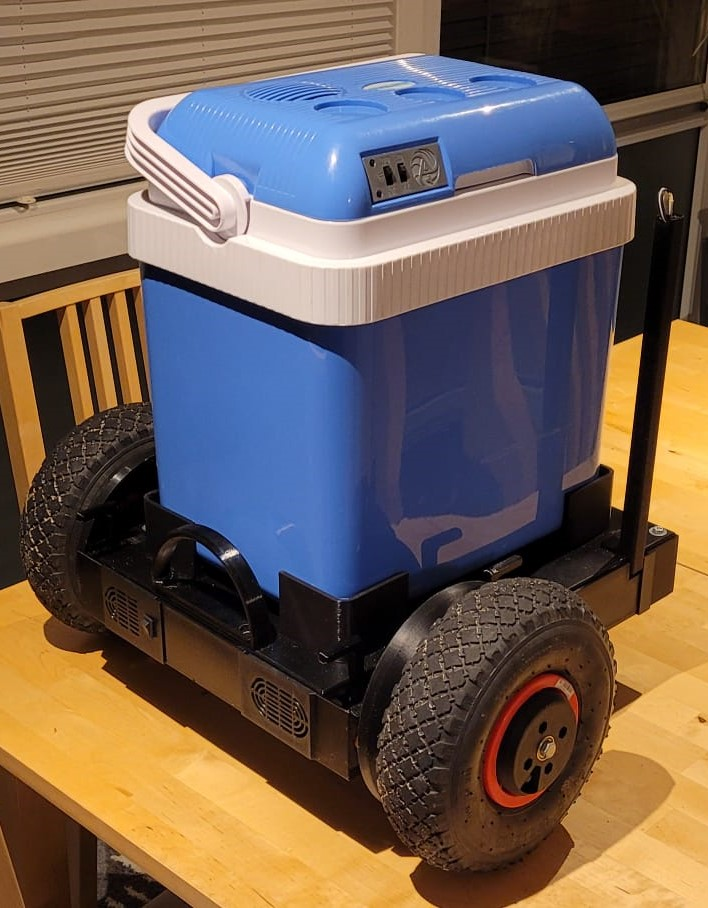
\includegraphics[width=8cm]{Robo_fertig.jpg}
\end{figure}

\vfill

\begin{tabular}{@{}p{5cm} l}
Studenten          &    Max Knauber\\
                           &    Matthias Gass\\
                           &    Fabian Schenker\\[2ex]
Fachbetreuer            &    Silvan Wirth\\[2ex]
\multicolumn{2}{@{}l}{Fachhochschule Nordwestschweiz, Hochschule für Technik}
\end{tabular}

\vspace*{4ex}
% Logo
\begin{tikzpicture}[remember picture,overlay,every node/.style={anchor=north west}]
  \node at (current page.north west) [xshift=0.5cm, yshift=-0.5cm] {
\includegraphics[width=20cm]{logo_neu.pdf}};
\end{tikzpicture}

\clearpage
			
%%---ABSTRACT-------------------------------------------------------------------
\pagestyle{plain}
\selectlanguage{ngerman}				%ngerman or english

\include{sections/00_zusammenfassung}
\section*{Vorwort / Dank}
\addcontentsline{toc}{section}{Vorwort / Dank}

Dieses Projekt hat gezeigt, wie wichtig eine gute Zusammenarbeit und Einsatz der fachlichen und sozialen Kompetenzen von jedem ist, die zum Erfolg von diesem Projekt beigetragen haban. \\
\\
Der FHNW danken wir für die Arbeitsmöglichkeiten im Labor, der Werkstatt und den Gruppenräumen.\\
\\
Herrn Silvan Wirth danken wir für die Begleitung während des Projekts und für die Beantwortung bei allfälligen Fragen.\\
\\
Wir danken uns gegenseitig für die gute Zusammenarbeit.\\
\\
Weiter geht unser Dank an alle weiteren Personen, welche hier nicht namentlich aufgelistet sind und uns bei dieser Projektarbeit ebenfalls unterstützt haben.

\section*{Rahmenbedingungen}
\addcontentsline{toc}{section}{Rahmenbedingungen}

\subsection*{Übersicht}
\begin{itemize}
    \item Zu realisierende Projekte können vorgeschlagen werden (Berücksichtigung gewisser Rahmenbedingungen)
    \item Bearbeitung in Zweier- oder Dreiergruppen
    \item Vorgabe SGL: lauffähige Produkte mit Aussenwirkung für Marketing
    \item Zuweisung von max. zwei Gruppen auf ein Projekt
    \item Austausch zwischen Gruppen möglich (Lösungsvarianz höher, Chance, dass ein lauffähiges Produkt entsteht, ist höher)
\end{itemize}
 

\subsection*{Rahmenbedingungen Projekte}
\begin{itemize}
    \item Enthält Merkmale eines mechatronischen Systems (Sensorik, Aktorik, Informationsverarbeitung (Rechner / Steuerung))
    \item Aktorik: physische Bewegung muss vorhanden sein
    \item User-Interface: optional, nicht zwingend
    \item Energieversorgung sinnvoll gelöst    
\end{itemize}

\subsection*{Qualifikationsziele und Kompetenzen}
\begin{itemize}
    \item Sachkompetenz:
    \begin{itemize}
        \item Verstehen und praktisches Anwenden der mechatronischen Modellbildung
    \end{itemize}
    \item Selbstkompetenz:
    \item \begin{itemize}
        \item Eigenständige Auswahl und Einsatz von Aktoren, Sensoren, Mikrorechner
    \end{itemize}
    \item Sozial-ethische Kompetenz:
    \begin{itemize}
        \item ein System vom Konzept bis zum funktionierenden Produkt entwickeln.
        \item mechatronisches Projekt im Team erfolgreich planen und durchführen.
        \item gruppendynamische Prozesse bei der Bearbeitung größerer Aufgaben innerhalb von Projektgruppen erfahren
    \end{itemize}
\end{itemize}

\subsection*{Unterstützung des Lernprozesses}
\begin{itemize}
    \item Aufwand gemäss Modulhandbuch: 15 h Präsenz, 45 h Selbststudium
    \item Anwenden des theoretischen Wissens aus der Vorlesung «Mechatronische Systeme» (und aller anderer vorgängiger Vorlesungen)
    \item Praktische Realisierung wird begleitet durch Dozenten.    
\end{itemize}

\subsection*{Verknüpfung in Modulgruppe Mechatronik III}
\begin{itemize}
    \item Fach «Mechatronische Systeme» wirkt auf Fach «Mechatronisches Labor»
    \item Inhalte und Methoden aus Vorlesung sollen angewendet werden
    \item Unterstützung bei Realisierung eines konkreten Projektes
\end{itemize}

\subsection*{Prüfungsbedingungen}
\begin{itemize}
    \item Leistungserfassung durch Präsentation und Bewertung des Projektes
    \item Termin: 10.01.2023	08:30 – 12:15
    \item Gewichtung: Schlussnote gemäss Bewertungsraster
\end{itemize}

\subsection*{Youtube-Videos / Mechatronik-Trinational Channel}
Zu den Projekten werden Videos gestaltet. Diese fliessen in die Bewertung der Projekte mit ein (siehe Bewertungsraster).\\
\\
Das Video Ihres Projektes muss «Youtube-konform» sein, z.B. sind die Musik-Copyrights zu beachten und wenn Sie (aus welchen Gründen auch immer) nicht im Video zu sehen sein wollen, dann sollten Sie sich auch nicht selbst aufnehmen.

\subsection*{Projektrahmen}
\begin{itemize}
    \item Kostendeckel CHF 200.-pro Projekt
    \item Kann ggf. bei marketingtechnischem Nutzen erhöht werden (nach vorheriger Absprache)
    \item Materialbeschaffung selbst zu organisieren
    \item Abrechnung über Sekretariat/Studiengangsleitung zum Ende des Semesters    
    \item Aufstellung mit Belegen und Kontoverbindung (IBAN) gemäss Formular
    \item Projekt muss vorgängig durch Dozenten genehmigt werden
    \item Arduino und/oder RaspberryPi wird abgegeben durch Labor (muss nicht in den Projektkosten berücksichtigt werden)
\end{itemize}

\subsection*{Laborzugang und Werkstattbenutzung}
\begin{itemize}
    \item Die Studierenden dürfen aus Sicherheits-und Versicherungsgründen das Labor Mechatronik Trinational / Campus Muttenz nicht unbegleitet (ohne Dozierenden) nutzen
    \item Zugang Labor Mechatronik Trinational gem. Unterrichtszeiten
    \item Werkstattaufträge (extern oder Hochschulen) sind vorgängig mit dem Dozierenden abzusprechen
    \item Kosten sind vorgängig zu klären und fliessen ins Projektbudget ein 
\end{itemize}

%%---TABLE OF CONTENTS-----------------------------------------------------------	
\pagestyle{empty}

\selectlanguage{ngerman}				%ngerman or english
\tableofcontents

\clearpage

%%---TEXT--------------------------------------------------------------------
\pagestyle{plain}
\pagenumbering{arabic}
\nocite{*}

\section{Einleitung}

\subsection{Sinn und Zweck des Dokuments}

\subsection{Vision (Inhalt und Ziele)}

\subsection{Definitionen und Abkürzungen}

\subsection{Ablage, Gültigkeit und Bezüge zu anderen Dokumenten}

\subsection{Verteiler und Freigaben}
\section{Aufgabenanalyse}

\subsection{Systemvoraussetzungen}
Unser System ist in sich geschlossen. Einzig für die Kommunikation mit dem Arduino werden wir uns einer App bedienen, die als User-Interface dienen soll. Auch soll das System Akkubetrieben sein, was einen vollen Akku und dementsprechend ein passendes Ladegerät voraussetzen.

\subsection{Problemdefinition}
Das schwere Schleppen von einer Kühlbox, soll mithilfe eines Mechatronischen Systems erleichtert werden. Die Idee war, die Schlepparbeit vom Auto zu einem Ort, an dem man sich mit der Familie oder mit Freunden niederlässt, etwas leichter zu gestalten. Dabei soll auf etwas lustiges und nützliches zurückgegriffen werden können.

\subsection{Systemabgernzung}
Um die Aufgaben für das Projekt einzugrenzen und eine Übersicht über die zu erreichenden Punkte zu erhalten, wurde eine Systemabgrenzung zur, von uns selbst gestellten, Aufgabenstellung erstellt. Diese Systemabgrenzung, angefangen mit dem Umsystem nach den PESTEL-Guidelines zeigt an sich weder Details noch Unerwartetes:

\begin{figure}[H]
    \begin{center}
    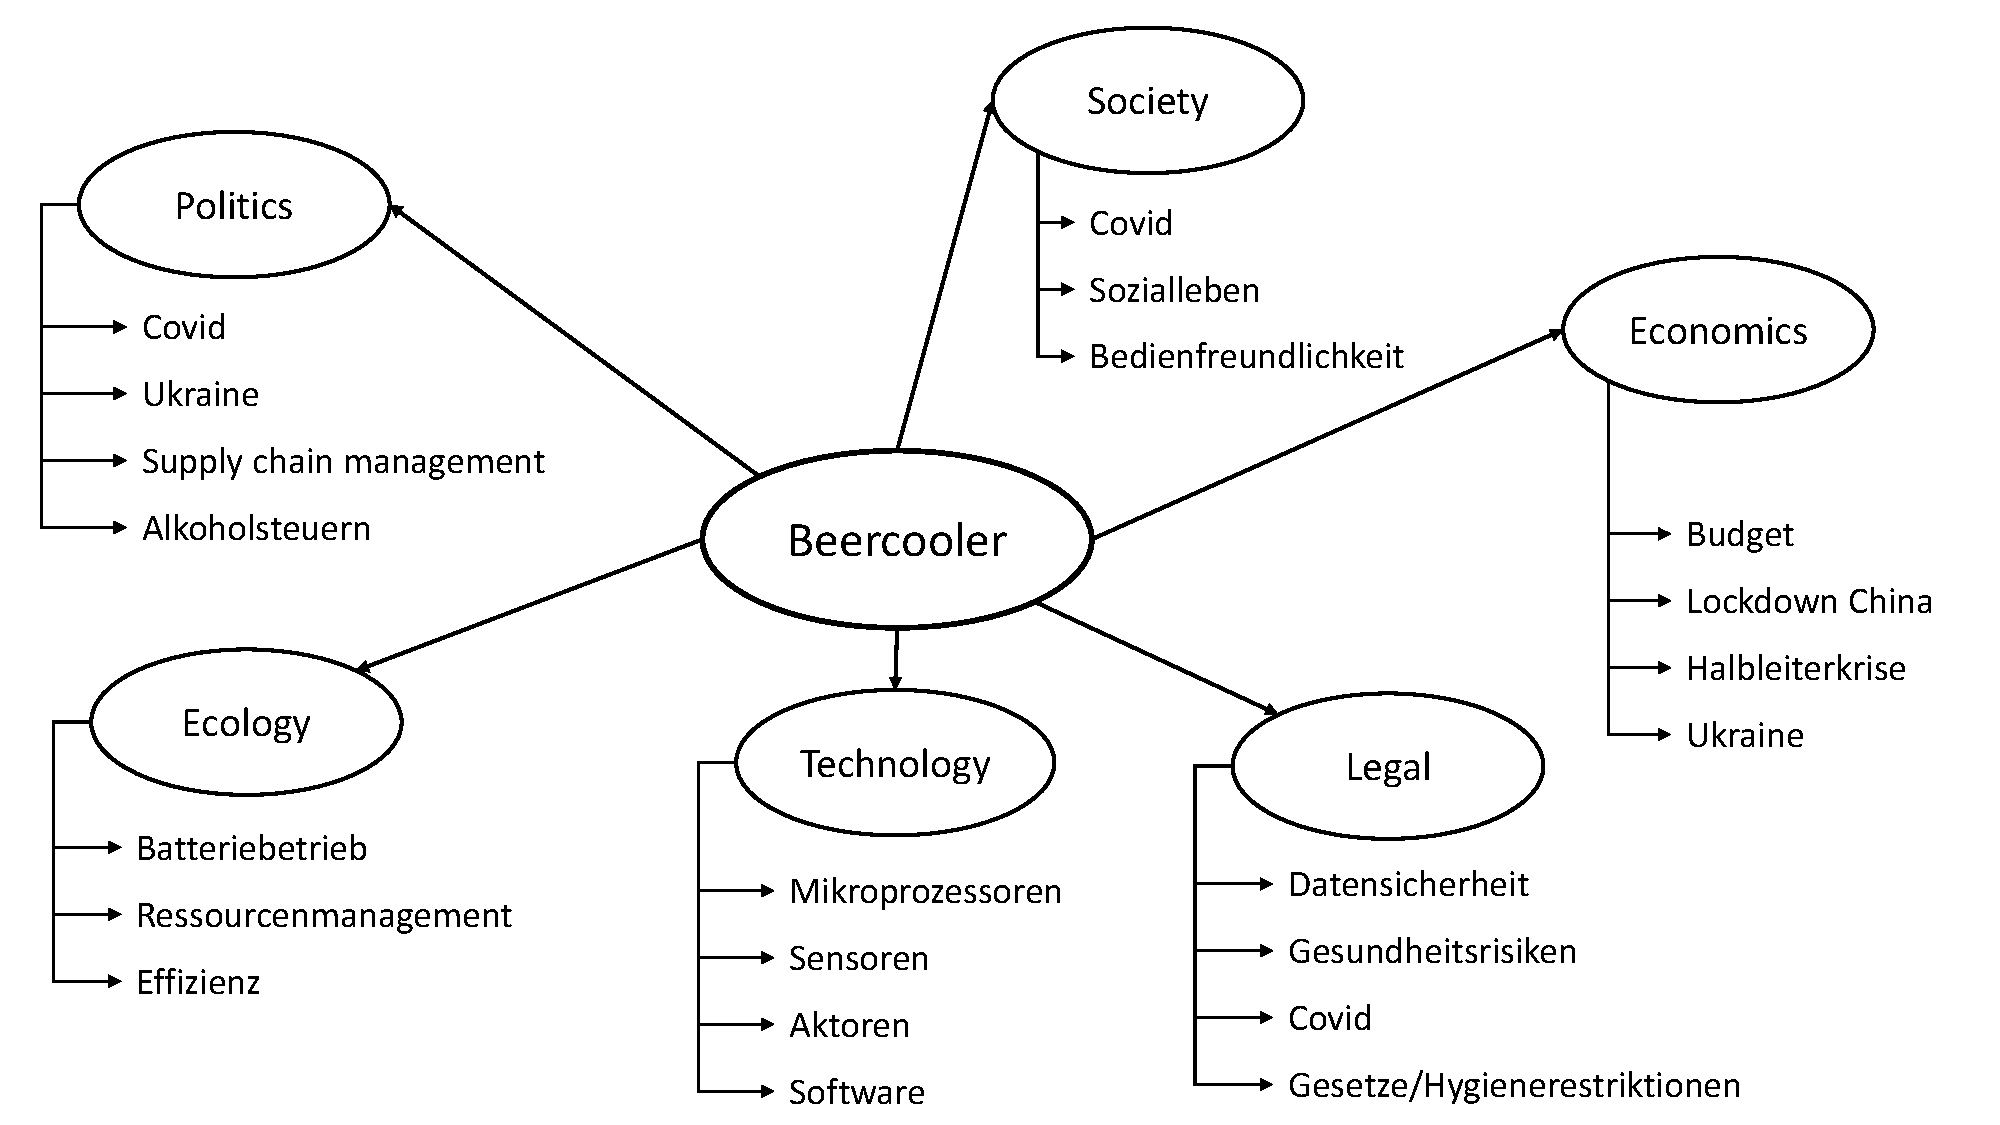
\includegraphics[width=\linewidth]{pestel.pdf}
    \end{center}
    \caption{Umfeld der Systemabgrenzung nach PESTEL}
\end{figure}

Bei genauerer Betrachtung des Umsystem kommt bereits etwas mehr zum Vorschein:

\begin{figure}[H]
    \begin{center}
    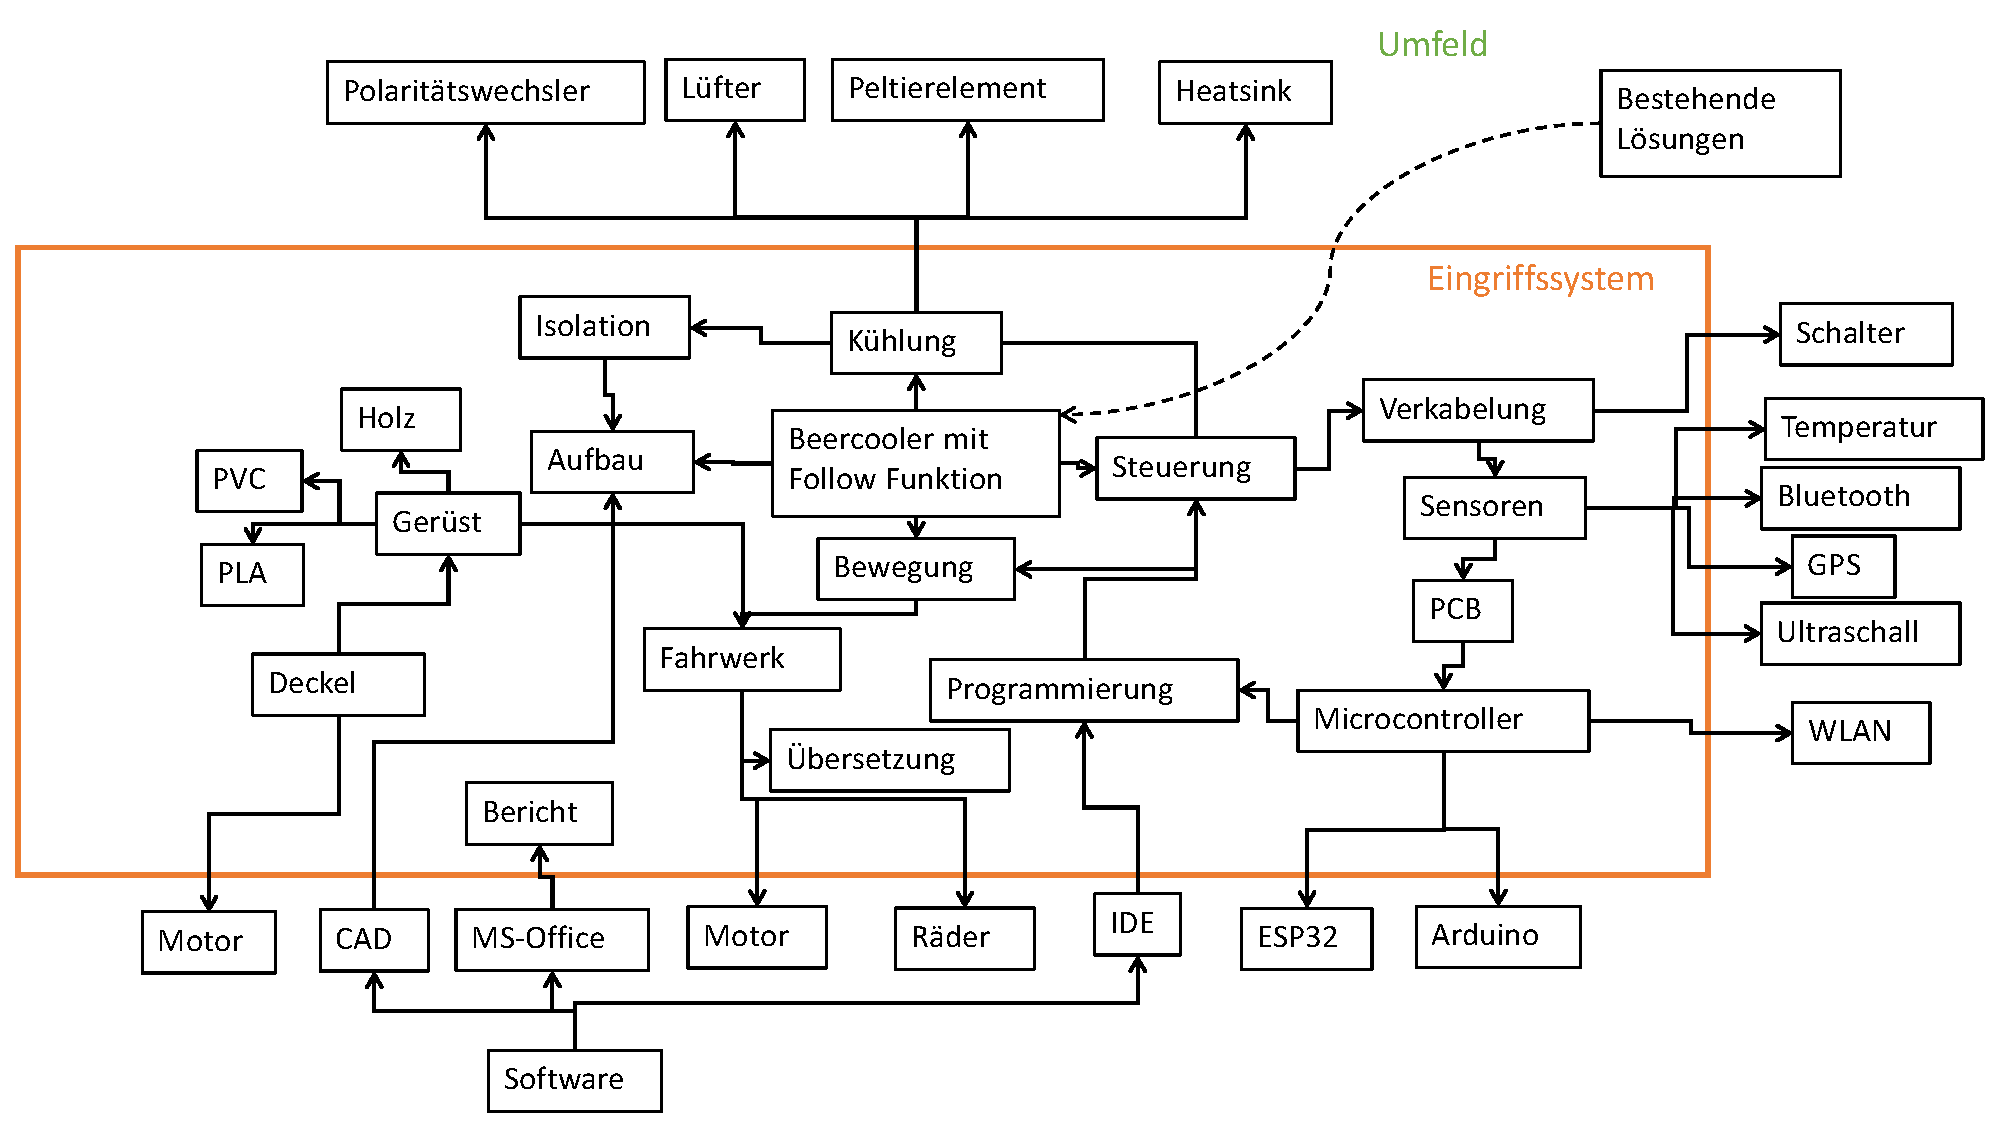
\includegraphics[width=\linewidth]{systemabgrenzung.pdf}
    \end{center}
    \caption{Systemabgrenzung}
    \label{fig:systemabgrenzung}
\end{figure}

Im Eingriffssystem sind alle Punkte enthalten für welche Eingriffe, Veränderungen und neue Konzepte im Rahmen der Aufgabenstellung zu erledigen sind. Das Umfeld beinhaltet die relevanten Teile für die Erarbeitung der Punkte im Eingriffssystem.

\subsection{Stärken- und Schwächenanalyse}
% Please add the following required packages to your document preamble:
% \usepackage{graphicx}
\begin{table}[H]
    \centering
    \caption{Stärken- und Schwächenanalyse}
    \resizebox{\columnwidth}{!}{%
    \begin{tabular}{|l|c|c|c|c|c|l|}
    \hline
    \textbf{Erfolgsfaktor} & \textbf{-{}-} & \textbf{-} & \textbf{0} & \textbf{+} & \textbf{+{}+} & \textbf{Begründung}                                 \\ \hline
    Arbeitszeiten          &             & X          &            &            &             & Zugang zum Labor ist eingeschränkt                  \\ \hline
    Betreuung              &             &            & X          &            &             & Nur während Laborzeiten                             \\ \hline
    Abgabetermin           &             &            &            & X          &             & Im Januar nach Ferien                               \\ \hline
    Innovation             &             &            & X          &            &             & Viele ähnliche Projekte   im Internet               \\ \hline
    Infrastruktur          &             &            &            & X          &             & Mechatronik Labor und FHNW   Werkstatt              \\ \hline
    Informatik Know-How    &             & X          &            &            &             & Kein Teammitglied aus   diesem Fachgebiet           \\ \hline
    Kommunikation          &             &            &            & X          &             & Ohne Probleme                                       \\ \hline
    Kosten                 &             &            & X          &            &             & Eher knapp                                          \\ \hline
    Materialbeschaffung    &             &            &            & X          &             & Selbstversorgung,   Abrechnung am Ende des Projekts \\ \hline
    Motivation             &             &            &            &            & X           & Sehr hoch, da eigen   ausgewähltes Projekt          \\ \hline
    Projekterfahrung       &             &            &            & X          &             & Nach Semester 4 und Stage   2 vorhanden             \\ \hline
    Sicherheit             &             &            & X          &            &             & LiPo Akku                                           \\ \hline
    Technisches Know-How   &             &            &            & X          &             & Unterschiedliche Stärken   der Teammitglieder       \\ \hline
    Zusammenarbeit         &             &            &            &            & X           & (noch) sehr gut privat   befreundet                 \\ \hline
    \end{tabular}%
    }
    \label{tab:my-table}
    \end{table}
\section{Zielformulierung}

\subsection{Ziele und Nutzen des Auftraggebers}
Der Auftraggeber wünscht sich ein lauffähiges Produkt, welches alle typischen Eigenschaften eines mechatronischen Systems (Sensorik, Aktorik, Informationsverarbeitung (Rechner / Steuerung)) enthält. Dabei sollen die Kenntnisse aus den früheren Semestern des Studiums angewendet werden.

\subsection{Ziele und Nutzen des Anwenders}
Der Anwender erwartet vom System eine simple Bedienung und eine unkomplizierte Benutzererfahrung. Er möchte möglichst wenig Schritte ausführen, um den Roboter zum Folgen zu bewegen. Wo immer ein Mensch mit Flip-Folps  geht, ausser ins Wasser natürlich, sollte der Roboter folgen können.

\subsection{Anforderungen}
Anforderungen an das System sind, dass sich eine Kühlbox auf Rädern selbst fortbewegen kann, wobei es leichtes Gelände bewältigen können muss, wie zum Beispiel eine Wiese. Des Weiteren sollen die darin aufbewahrten Getränke deutlich unter Lufttemperatur temperiert werden.

\subsection{Zielkatalog}
\begin{table}[H]
    \centering
    \caption{Zielkatalog}
    \label{tab:Zielkatalog}
    \resizebox{\columnwidth}{!}{%
    \begin{tabular}{|llllll|}
    \hline
    \multicolumn{1}{|l|}{\textbf{Objekt}} & \multicolumn{1}{l|}{\textbf{Eigenschaft}}                                                        & \multicolumn{1}{l|}{\textbf{Ausmass}} & \multicolumn{1}{l|}{\textbf{Zeitpunkt}} & \multicolumn{1}{l|}{\textbf{Zielart}} & \textbf{Priorität} \\ \hline
    \multicolumn{6}{|l|}{\textbf{Level 1}}                                                                                                                                                                                                                                                  \\ \hline
    \multicolumn{1}{|l|}{Gerüst}          & \multicolumn{1}{l|}{Aufbau des Roboters   mit Fahrwerk, Halterung für Kühlbox und Elektronik}    & \multicolumn{1}{l|}{zusammengebaut}   & \multicolumn{1}{l|}{KW 46}              & \multicolumn{1}{l|}{M}                & -                  \\ \hline
    \multicolumn{1}{|l|}{Follow-Funktion} & \multicolumn{1}{l|}{Roboter kann   autonom jemandem nachfahren}                                  & \multicolumn{1}{l|}{erreicht}         & \multicolumn{1}{l|}{KW 50}              & \multicolumn{1}{l|}{M}                & -                  \\ \hline
    \multicolumn{1}{|l|}{isolierte Box}   & \multicolumn{1}{l|}{Eine Kiste, welche   die Innentemperatur von der Aussentemperatur isoliert.} & \multicolumn{1}{l|}{}                 & \multicolumn{1}{l|}{KW 44}              & \multicolumn{1}{l|}{M}                & -                  \\ \hline
    \multicolumn{1}{|l|}{Kühlen}          & \multicolumn{1}{l|}{Die isolierte Box   soll gekühlt werden}                                     & \multicolumn{1}{l|}{< 5 °C}           & \multicolumn{1}{l|}{KW 46}              & \multicolumn{1}{l|}{R}                & 100                \\ \hline
    \multicolumn{1}{|l|}{Akku}            & \multicolumn{1}{l|}{Der Akku soll für   3h aktive Kühlung und 1h Fahren ausreichen}              & \multicolumn{1}{l|}{erreicht}         & \multicolumn{1}{l|}{KW 48}              & \multicolumn{1}{l|}{M}                & -                  \\ \hline
    \multicolumn{1}{|l|}{Kapazität}       & \multicolumn{1}{l|}{Es soll mindestens   Platz für 12 0.5 L Dosen haben}                         & \multicolumn{1}{l|}{erreicht}         & \multicolumn{1}{l|}{KW 44}              & \multicolumn{1}{l|}{M}                & -                  \\ \hline
    \multicolumn{6}{|l|}{\textbf{Level 2}}                                                                                                                                                                                                                                                  \\ \hline
    \multicolumn{1}{|l|}{Wechsel Akku}    & \multicolumn{1}{l|}{Akku soll   auswechselbar sein}                                              & \multicolumn{1}{l|}{erreicht}         & \multicolumn{1}{l|}{KW 48}              & \multicolumn{1}{l|}{W}                & 40                 \\ \hline
    \multicolumn{1}{|l|}{Deckel}          & \multicolumn{1}{l|}{Der Deckel soll sich   automatisch öffnen können}                            & \multicolumn{1}{l|}{erreicht}         & \multicolumn{1}{l|}{KW 49}              & \multicolumn{1}{l|}{W}                & 30                 \\ \hline
    \multicolumn{1}{|l|}{All-Terrain}     & \multicolumn{1}{l|}{Der Roboter soll   auch über kleinere Hindernisse fahren können}             & \multicolumn{1}{l|}{5cm Schwelle}     & \multicolumn{1}{l|}{KW 49}              & \multicolumn{1}{l|}{O}                & 30                 \\ \hline
    \multicolumn{1}{|l|}{Federung}        & \multicolumn{1}{l|}{Einbau einer   Federung/Dämpfung}                                            & \multicolumn{1}{l|}{erreicht}         & \multicolumn{1}{l|}{}                   & \multicolumn{1}{l|}{W}                & 20                 \\ \hline
    \multicolumn{6}{|l|}{\textbf{Level 3}}                                                                                                                                                                                                                                                  \\ \hline
    \multicolumn{1}{|l|}{Leine}           & \multicolumn{1}{l|}{Leine, an der der   Roboter gezogen werden kann, falls der Akku leer ist.}   & \multicolumn{1}{l|}{erreicht}         & \multicolumn{1}{l|}{}                   & \multicolumn{1}{l|}{W}                & 30                 \\ \hline
    \multicolumn{1}{|l|}{Variable Temp.}  & \multicolumn{1}{l|}{Die Temperatur in   der Kühlbox soll variabel geregelt werden}               & \multicolumn{1}{l|}{erreicht}         & \multicolumn{1}{l|}{}                   & \multicolumn{1}{l|}{W}                & 10                 \\ \hline
    \multicolumn{1}{|l|}{Wärmen}          & \multicolumn{1}{l|}{Die Isolierte Box   soll heizbar sein}                                       & \multicolumn{1}{l|}{Warm 50° C}       & \multicolumn{1}{l|}{}                   & \multicolumn{1}{l|}{W}                & 40                 \\ \hline
    \end{tabular}%
    }
    \end{table}

\subsection{Benutzer / Zielgruppe}
\begin{table}[H]
    \centering
    \caption{Benutzer / Zielgruppe}
    \label{tab:Zielgruppe}
    \begin{tabular}{|l|l|l|}
    \hline
    \rowcolor[HTML]{E0E0E0} 
    \textbf{Zielgruppe} & \textbf{Name}                & \textbf{Beschreibung}            \\ \hline
    Stakeholder         & FHNW, Silvan Wirth           & Ansprechperson / Auftraggeber    \\ \hline
    Anwender            & Prof. Dr. Robert   Alard     & Kunde                            \\ \hline
    Zielgruppe          & Studenten/Familien/Marketing & Potentielle Studieninteressierte \\ \hline
    \end{tabular}
    \end{table}
\section{Konzepterarbeitung}

\subsection{Morphologischer Kasten}

\subsection{Ressourcen Personell und Materiell}

\subsection{Projektablauf}

\subsection{Grobschätzung des Aufwands}

\section{Konzeptbeschreibung}

\subsection{Systembeschreibung}

\subsection{Grundsätzlicher Aufbau (Blockschaltbild)}

\subsection{Use-Case Übersicht}

\subsection{Vergleich mit bestehenden Lösungen}

\subsection{Nicht-funktionale Anforderungen}
\section{Schnittstellen}

\subsection{Übersicht}
Da in diesem Projekt nur ein Mikrokontroller verwendet wird, halten sich die Hardwareschnittstellen in Grenzen.

\subsection{Hardwareschnittstellen}
Als Hardwareschnittstellen kommen lediglich Jumper-Kabel zum Einsatz, sowohl für die Datenübertragung als auch für die Versorgungsspannung. Dafür soll möglicherweise ein Kabelbaum zum Einsatz kommen. \\
\\
Wir führen hier auch noch die Motorentreiber auf. Sie nutzen ein PWM-Signal, durch welches sie die ihnen zur Verfügung gestellte 24V Spannung in unterschiedlicher Stärke an die Motoren weitergeben. 

\begin{figure}[H]
    \begin{center}
    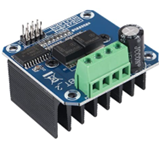
\includegraphics[width=4cm]{Hardware-Schnittstelle_PWM.png}
    \end{center}
    \caption{Motorentreiber}
\end{figure}

\subsection{Softwareschnittstellen}
Die Kommunikation zwischen den Sensoren und dem Arduino soll über das UART- und das I2C- Protokoll laufen. Das I2C-Protokoll benutzt die SCL- und SDA- Pins (A4- und A5 auf dem Arduino UNO), welche vom Kompass-Modul benutzt werden soll.\\
\\
Das GPS-Modul und das Bluetooth-Modul sollen über ein UART-Protokoll mit dem Arduino kommunizieren. Dafür sind alle Pins mit PWM-Funktion auf dem Arduino ausreichend. \\
\\
Die Motorentreiber erhalten ein 5V PWM-Signal welches sie in ihrer Ausgangsspannung, in unserem Fall 24V, weitergeben.

\section{Mechanik}

\subsection{Mechanische Struktur}
Das Grundgerüst des Beercoolers besteht aus 2 MDF-Holzplatten, welche über Stützen miteinander verschraubt werden, sodass zwischen ihnen ein Hohlraum entsteht. In diesem Hohlraum ist Platz für sämtliche Elektronik, die Motoren, den Mikrokontroller und den Akku. Auf der Rückseite des Roboters befindet sich an der oberen Platte ein Rad mit neutraler Lenkung, am vorderen Ende befinden sich zwei angetriebene Räder.\\
\\
Auf der oberen Platte befinden sich 4 Führungen, in welchen die Kühlbox zu platzieren ist. Die elektrische Verbindung ist in die Platte eingearbeitet und stellt eine einwandfreie Verbindung sicher. Die Kühlbox lässt sich dann auf Heizen oder Kühlen einstellen.

\begin{figure}[H]
    \begin{center}
    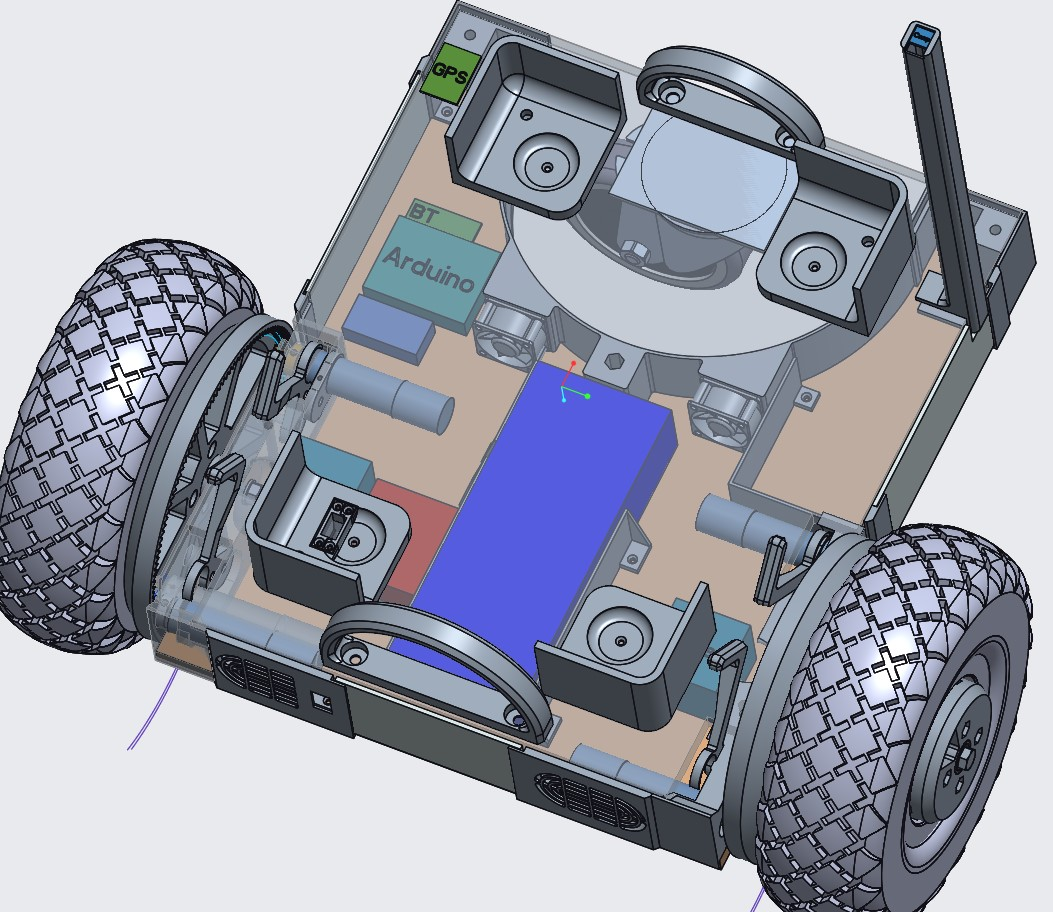
\includegraphics[width=8cm]{Aufbau.jpg}
    \end{center}
    \caption{Aufbau im CAD}
\end{figure}

\subsection{Führungen / Getriebe}
Die Fortbewegung wird über 4 Brushless DC-Motoren von Faulhaber und ein Zahnradpaar gewährleistet. Der Kraftschluss geschieht über ein direkt auf der Motorwelle montiertes kleines, und über ein Innenverzahntes grosses Zahnrad, welches mit dem Rad verschraubt ist\\

\begin{figure}[H]
    \begin{center}
    \includegraphics[width=6cm]{Führungen Getriebe_Zahnrad.jpg}
    \end{center}
    \caption{3D gedruckte Zahnräder}
\end{figure}

Die Motoren sind zudem über einen Hebelmechanismus zurückziehbar, wodurch es möglich ist den Roboter auch ohne den Einsatz der Motoren so reibungsfrei wie möglich zu bewegen. 

\begin{figure}[H]
    \begin{center}
    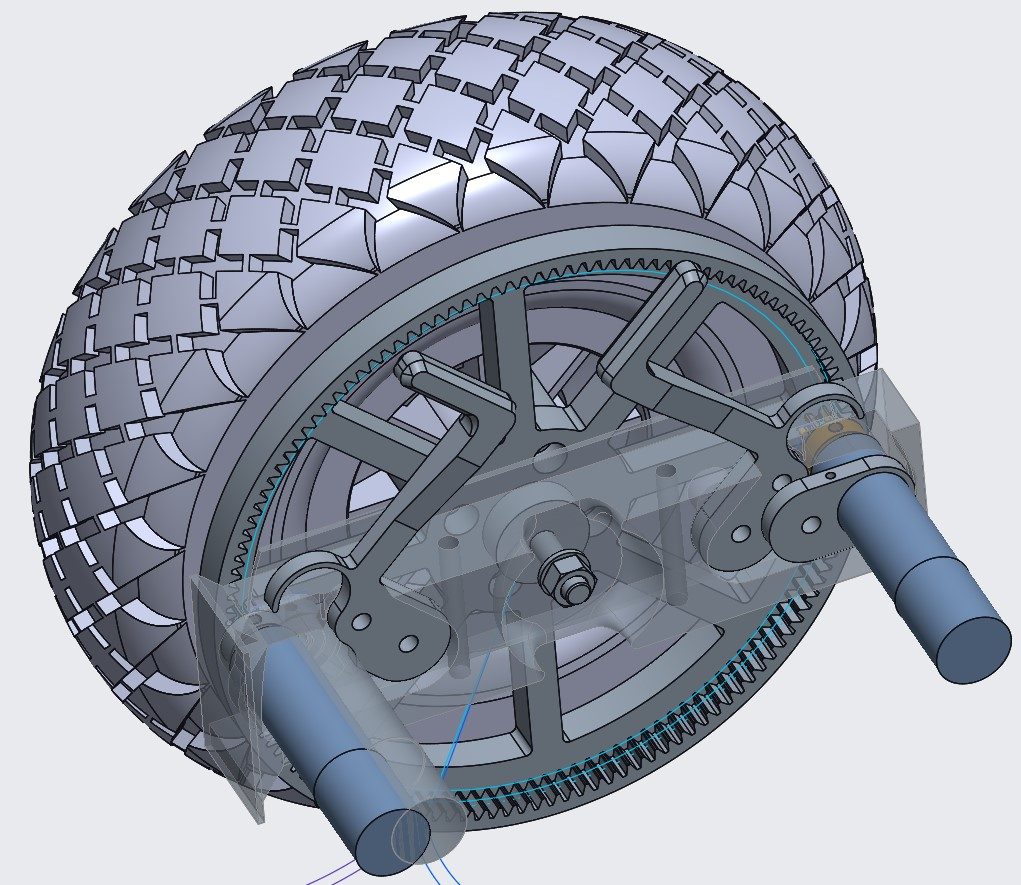
\includegraphics[width=6cm]{rad_asm.jpg}
    \end{center}
    \caption{Rad mit Aufnahme und Hebelmechanismus}
\end{figure}

Um eine reibungsfreie Bewegung zu Erreichen, wurden bei den angetriebenen Rädern Kugellager eingebaut. Hier ist es wichtig auf den korrekten Einbau der Kugellager zu achten, damit durch den Zusammenbau der Baugruppe keine überhöhten axiale Kräfte auf das Lager wirken. Dies kann zum versagen der Lager führen.
\section{Sensoren}

\subsection{Sensor xy}

\section{Aktoren}

\subsection{Motoren}
Als einzige steuerbare Aktoren dienen uns DC Motoren von Faulhaber mit einem integrierten Reduktionsgetriebe. Es werden 2 pro Rad zum Einsatz kommen um ausreichend Drehmoment erzielen zu können.

\begin{figure}[H]
    \begin{center}
    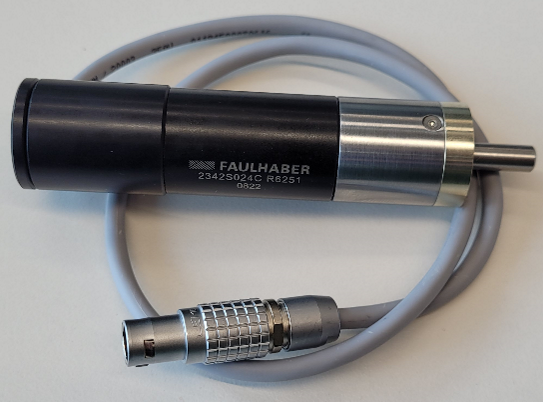
\includegraphics[width=6.3cm]{Aktoren_Motor.png}
    \end{center}
    \caption{Motor}
\end{figure}

\subsection{Peltier Element}
Das Peltier-Element in der Kühlbox erzeugt eine Temperaturdifferenz, sobald man eine Spannung daran anlegt. Mit 2 Lüftern und 2 Kühlelementen, welche in der gekauften Kühlbox bereits vorhanden sind, ist es möglich sowohl zu heizen als auch zu kühlen. \\
\\
Da die Endtemperatur von der Aussentemperatur abhängt, lässt sich hier lediglich eine Temperaturdifferenz sinnvoll definieren, welches ich auf 10-15 Grad festlegen lässt.
\begin{figure}[H]
    \begin{center}
    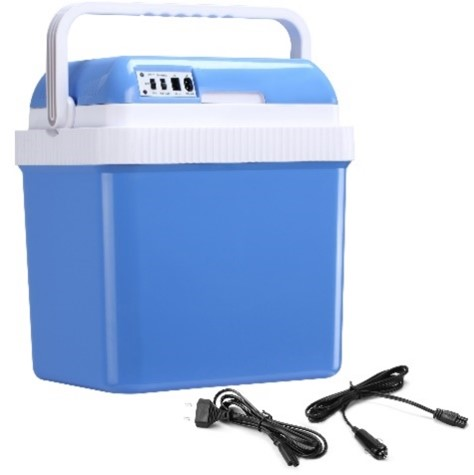
\includegraphics[width=5.5cm]{Aktoren_Peltier Element.jpg}
    \end{center}
    \caption{Kühlbox}
\end{figure}
\section{Elektronik}

\subsection{Schnittstellenplatine}

\subsection{Messwertverarbeitung}

\subsection{Leistungsteil}

\section{Informationsverarbeitung}

\subsection{Digitalrechner}
\begin{figure}[H]
    \begin{center}
    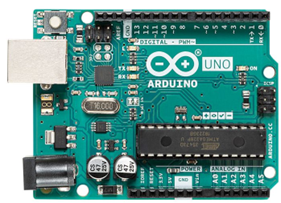
\includegraphics[width=7cm]{Digitalrechner_Arduino Uno.png}
    \end{center}
    \caption{Arduino}
\end{figure}

Auf dem Arduino ist ein Atmega328 Mikroprozessor verbaut. Dieser ist auf einer Platine beschaltet. Das Programm kann mit der Arduino IDE direkt über eine serielle Schnittstelle auf den Arduino geladen werden. Es wird also kein externes Kompiliergerät benötigt. Mit der Arduino IDE lassen sich auf dem Arduino UNO rund 20 Pins programmieren. Bei einem Arduino UNO sind folgende Anschlüsse vorhanden:

\begin{itemize}
    \item 13x digital Pins 
    \item 3x Timer 
    \item 6x PWM Pins 
    \item SDA und SCL Pins 
    \item 6x analog Pins 
    \item MISO MOSI Pins
\end{itemize}

Benutzt werden hierbei 5 der PWM-Pins, 4 der normalen Digital-Pins, die SDA- und SCL-Pins. Der USB-Anschluss wird lediglich zur Übertragung des Programms und zur Überwachung der korrekten Funktion während der Entwicklung benötigt.


\subsection{Steuerung}
Die Steuerung des Roboters erfolgt lediglich über die Motoren, welche mit unterschiedlichen PWM-Signalen neben vorwärtsn nach links und nach rechts gesteuert werden. 

\subsection{Regelung}
Die Regelung erfolgt über eine Kombination aus Kompass, den GPS-Koordinaten des Handys und den GPS-Koordinaten des GPS-Moduls, welches mit dem Arduino verbunden ist. Mittels der 2 Koordinatensets soll die Distanz zwischen den beiden Punkten errechnet werden, der Kompass gibt schliesslich die Richtung an, in welche es sich zu drehen gilt. Sobald die Distanz unter einen gewissen Schwellenwert fällt, wird die Position des Handy-GPS wieder überprüft und der Prozess beginnt von vorne. 
\\ \\
Das Fundament für die Berechnung bildet die Natur des GPS-Koordinatensystems. Dieses hat seinen «Nullpunkt» am Schnittpunkt zwischen Äquator und dem Null-Meridian, der Nord-Süd Achse durch Greenwich, Vereinigtes Königreich. 
Ein GPS-Standpunkt ist stets in Latitude und Longitude unterteilt. Die Latitude gibt den Winkel zwischen der Äquatorlinie und dem Standpunkt an und die Longitude gibt den Winkel zwischen Nullmeridian und dem Standpunkt an.
\\ \\
Dank der Haversine Formel 

\[a=sin^{2}\left ( \frac{p_{2}.lat-p_{1}.lat}{2} \right )+cos\left ( p_{1}.lat \right )*cos\left ( p_{2}.lat \right )*sin^{2}\left ( \frac{p_{2}.lon-p_{1}.lon}{2} \right )\]
\[b=2*atan2\left ( \sqrt{a},\sqrt{1-a} \right )\]
\[d=R*b\]

lässt sich die Distanz zwischen 2 GPS-Punkten relativ leicht berechnen. R ist der Erdradius von 6371 km. \\ \\
Über folgende Formel:

\[\beta = atan2(sin\left ( p_{2}.lon-p_{1}.lon \right )*cos\left ( p_{2}.lat \right ), cos\left (p_{1}.lat  \right )*sin\left ( p_{2}.lat \right )-\] 
\[sin\left ( p_{1}.lat \right )*cos\left (p_{2}.lat  \right )*cos\left ( p_{2}.lon-p_{1}.lon \right ))\]

lässt sich indes der Winkel zwischen der Nord-Süd-Achse durch Punkt 1 und der Achse, welche durch die beiden Punkte geht, berechnen. Man nennt dies die Peilrichtung, oder Bearing.
\\ \\
Wenn man nun den Winkel, resp. die eigene Ausrichtung gegenüber dem Nordpol kennt, zum Beispiel durch einen Kompass, kann man diesen Winkel von der Peilrichtung abziehen und erhält den Winkel, um den man sich drehen muss, um in Richtung des zweiten Punktes zu zeigen.

\section{Software}

\subsection{Softwareverweise}

\section{Benutzerinterface}

\subsection{Layout}
Das Layout beruht auf der gegebenen Blynk Oberfläche und einer Auswahl an verfügbaren Widgets. Wir mussten dabei auf eine Legacy Version der App zurückgreifen, da die möglichkeit zur Verbindung mit Bluetooth eingestellt wurde.

\begin{figure}[H]
    \begin{center}
    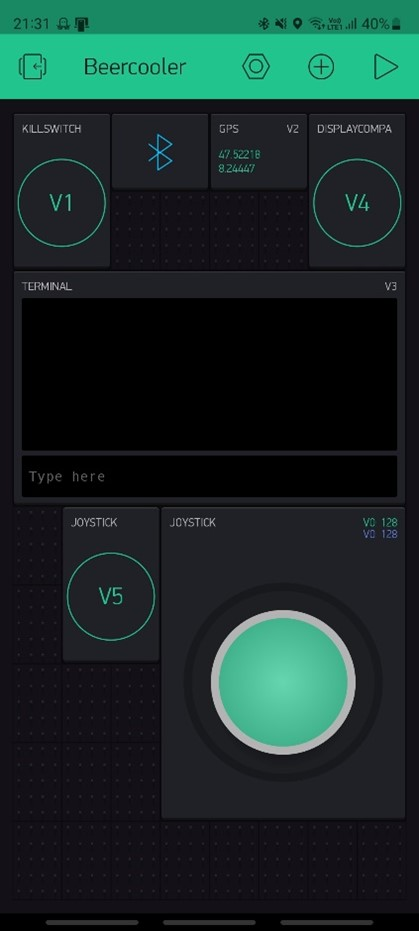
\includegraphics[width=5cm]{Layout_BlynkApp.jpg}
    \end{center}
    \caption{Layout in der Blynk App}
\end{figure}

Es soll mindestens ein Killswitch, eine Bluetooth-Verbindung, ein GPS-Stream und ein Terminal darin enthalten sein.

\subsection{Funktionen}
Über den Killswitch soll der Roboter in den «Fahren»-Modus versetzt werden können und diesen wieder verlassen. Das Bluetooth- und GPS-Widget dienen lediglich dem Informationsaustausch zwischen dem Ardu-ino und der App. Der Terminal soll schliesslich die Möglichkeit bieten, GPS-Koordinaten direkt dem Arduino zuzuführen, zu welchen er fahren soll.
\section{Schlussbemerkungen}

\lipsum[28]


%%---BIBLIOGRAPHY-------------------------------------------------------
{\sloppypar
\printbibliography[title=Quellenverzeichnis]
}

%%---APPENDIX----------------------------------------------------------
\section*{Ehrlichkeitserklärung}
\addcontentsline{toc}{section}{Ehrlichkeitserklärung}

Hiermit erkläre ich, die vorliegende [Projektarbeit, Individualarbeit, Bachelorarbeit etc.] selbständig und nur unter Benutzung der angegebenen Quellen verfasst zu haben. Die wörtlich oder inhaltlich aus den aufgeführten Quellen entnommenen Stellen sind in der Arbeit als Zitat bzw. Paraphrase kenntlich gemacht. Diese [Studien-/Projektarbeit/Bachelor Thesis] ist noch nicht veröffentlicht worden. Sie ist somit weder anderen Interessierten zugänglich gemacht noch einer anderen Prüfungsbehörde vorgelegt worden.

\vspace*{4ex}

Windisch, tt. Monat 20jj

\vspace*{4ex}

{\renewcommand{\arraystretch}{2}
\begin{tabular}{@{}>{\bf}ll}
Name: & Pia Musterfrau\\
Unterschrift: & \\[6ex]
Name: & Michael Mustermann\\
Unterschrift: & \\
\end{tabular}
\begin{appendix} %Anhang

\listoffigures
\listoftables

\pagebreak

\section{Anhang / Ressourcen}

\subsection{Impressum}
Datum der Erstellung der Dokumentation: Herbst und Winter 2022/2023\\
\\
© Fachhochschule Nordwestschweiz, Studiengang Mechatronik Trinational, 2023

\subsection{Quellcode}

\lstinputlisting[language=C++,frame=single,label=coolercode,caption=Programm des Roboters]{code/Cooler_FaMaMa.ino}
\lstinputlisting[frame=single,label=coolerdefinition,caption=Definitionen für das Programm]{code/CoolerDefinitions.h}

\end{appendix}


%%---NOTES for DEBUG---------------------------------------------------------------------
%\newpage
%\listoftodos[\section{Todo-Notes}]
%\clearpage

\end{document}